
%(BEGIN_QUESTION)
% Copyright 2010, Tony R. Kuphaldt, released under the Creative Commons Attribution License (v 1.0)
% This means you may do almost anything with this work of mine, so long as you give me proper credit

Calculate the maximum amount of power supply voltage allowed across a 47 $\mu$F capacitor to limit the energy stored in that capacitor to a maximum of 60 mJ.

\vskip 10pt

$$\includegraphics[width=15.5cm]{i04738x01.eps}$$

$V_{max}$ = \underbar{\hskip 50pt} V

\vskip 10pt

Next, write the manipulated version of the capacitive energy storage equation, solving for voltage ($V$).

\vskip 10pt

$V$ = 

\underbar{file i04738}
%(END_QUESTION)





%(BEGIN_ANSWER)

$V_{max}$ = \underbar{\bf 50.529} V

\vskip 10pt

$V = \sqrt{2 U \over C}$

%(END_ANSWER)





%(BEGIN_NOTES)

{\bf This question is intended for exams only and not worksheets!}

%(END_NOTES)


